\subsection{Singleton}
The program uses a server to gather and record the data from the eye tracking camera. This server is constantly running and there should only be one instance of this class running so that we do not have multiple servers running and all the data is pulled consistently from one location. The server will thus need to follow the singleton design pattern. The singleton design pattern is a creational design pattern that is used when only one instance of the object should be created for the application. This will provide the solution of only one server object being created at time. It will check whether an instance of the requested object is created and if it is the object is referenced and not recreated and therefore there can only be one instance of the class created.



%\subsection{Extensibility pattern}
%The program is comprised of many different modules to increase the re-usability of the different developed code. The different modules will need to work together to perform all the tasks that the program is required to carry out. The extensibility pattern helps to achieve this. The extensibility pattern provides a framework for the inclusion of other modules into the program. This is achieved through C\# and its ability to create DLL (Dynamic Link library) for use in another solution. This allows us to very easily add functionality and will also allow the fixing and enhancing of the application at a later stage without affecting any other working modules. Meaning that modules can be easily added and removed from the system with little negative affect.
%

\subsection{Flyweight}
The program has data that needs to be shared amongst modules and that also needs to be used throughout the system. This is achieved by use of the flyweight pattern. The application requires all system and model settings to be created, saved and eventually used by the rest of the modules within the system. These variables are static and are defined as internal so that only the program can access the stored setting values. This ensures that all the modules are able to read and change the shared memory resource.


	\begin{figure}[!ht]
		\centering
		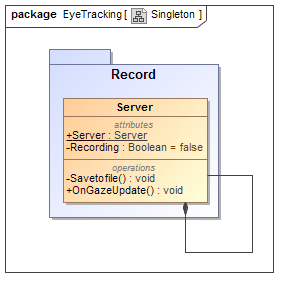
\includegraphics[scale=0.5]{Diagrams/Class_Diagram__Singleton.png}
		\caption{Singleton}
	\end{figure}



\begin{figure}[!ht]
		\centering
		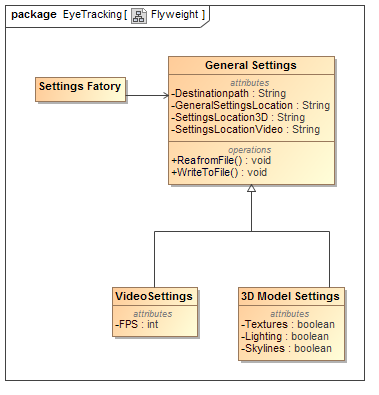
\includegraphics[scale=0.5]{Diagrams/Class_Diagram__Flyweight.png}
		\caption{Flyweight}
	\end{figure}


%\subsection{Model-View-Controller} 
%\begin{flushleft}
%The project can easily be split as: User, Interface and, Background Calculations. The user interacts %with the Interface, the program that will be executed, handling the eye tracking. The interface will %convert the received data into a format that the data processing section can work with. The data %processing section will take render out/back the heat maps generate from the users focus.

%It is with this in mind that the Model-View-Controller(MVC) design pattern will be used.
%The MVC separates the data model, user interface, and control logic which is exactly what we want. We %want the user to be able to use our system without having to know how it works. Only the basics %should be available i.e record, printing out texture/model.
%\end{flushleft}